\section{Introduction to Bipolar Junction Transistors}
\label{lab_bjt}

%\makelabheader %(Space for student name, etc., defined in master.tex)

\bigskip

\begin{enumerate}[wide]

\item Build the circuit drawn below, which includes a 2N3904 npn bipolar junction transistor.  Measure the DC current through the base, collector, and emitter leads of the transistor.  (To minimize the effect of your DMM on the circuit, use the ``mA'' scale where possible.)  What is the ratio of $I_E/I_B$?  (You should get a ratio of about 100.)  Where is all the current in the emitter coming from?
\begin{center}
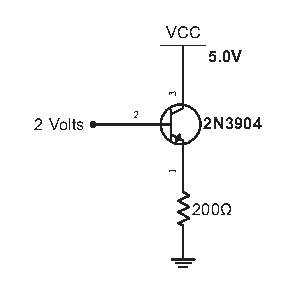
\includegraphics{bjt/first_bjt_test_circuit.eps}
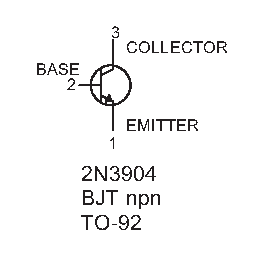
\includegraphics{appendices/pinouts/2N3904_pinout.eps}
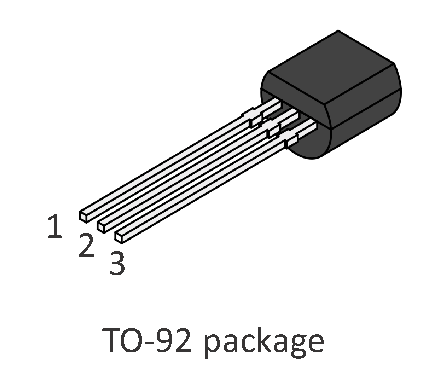
\includegraphics[width=1.3in]{appendices/pinouts/TO-92_package_pinout.eps}
\end{center}

\item What happens to the voltage across the 200 $\Omega$ resistor as you raise the voltage of the base (carefully) to 3 volts?  3.5 volts?  4 volts?  What is the voltage difference $V_B-V_E$?

\item By connecting the base of the transistor to a DC voltage as you did in parts 1 and 2, you are effectively using the transistor as a switch.  That is, by turning the DC base voltage on and off, you control current flow through the collector and the emitter.  How fast does current turn on in the emitter when you connect the base to a DC voltage?  (Measure it!)  How does this compare with the switching speed of the relay switch you measured?  (Note: You may not be able to get an accurate measurement of the delay time, but you should at least be able to set an upper limit.)

\item How does the size of the current $I_B$ compare to the current in the coil of the relay switch from the Lab~\ref{lab_relays}?

\item In the circuit below, the output of an op-amp is being used to light a red LED.  (Perhaps this is the last stage of some other more complicated project.)  This circuit should work just fine. Build it and verify that the output voltage of the op-amp and the current through the LED are what they should be. 
\begin{center}
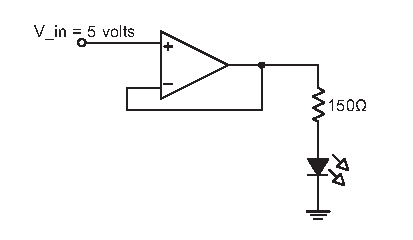
\includegraphics{bjt/buffer_one_led.eps}
\end{center}

\pagebreak[3]
\item Now suppose that you want to use the op-amp's output to power three additional LEDs in parallel, as shown below.  What is the maximum output current of the LM324?  How is the current through the first LED affected by the addition of the other three?
\begin{center}
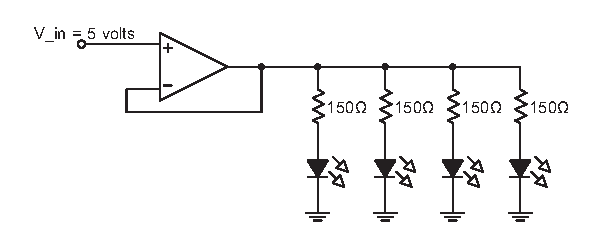
\includegraphics{bjt/buffer_four_leds.eps}
\end{center}

\item The circuit below shows one way to fix the problem you just found, using a transistor as an ``emitter follower amplifier.''  Now what is the current through each LED?  What is the voltage at the emitter, $V_E$?  What is the current $I_B$?  (BTW: No worries, the LM324 will be perfectly happy with 10~V for its positive power supply.)
\begin{center}
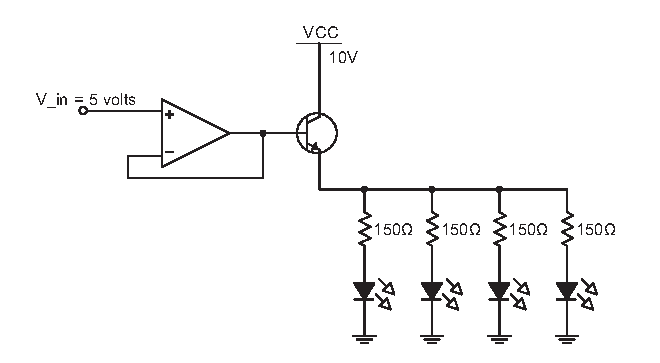
\includegraphics{bjt/emitter_follower1.eps}
\end{center}

\item The circuit above has a problem, that the emitter of the transistor is always about 0.7 volts lower than the base, so that the voltage across the load is always 0.7 volts lower than you really want it to be.  The circuit below shows an improved version of what you just built.  In the circuit below, what is $V_E$, and what is the $V_{OUT}$ of the op-amp?  And finally, what is the current through each LED?  (Clever, eh?)  
\begin{center}
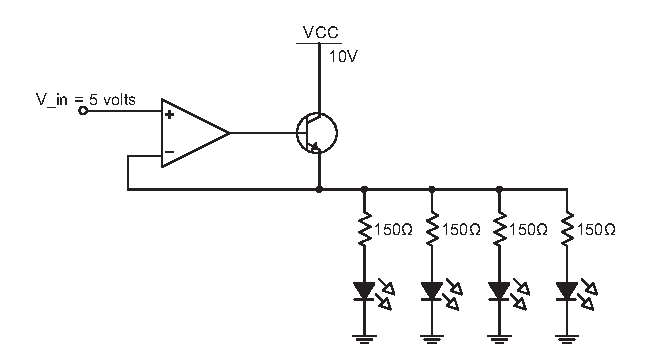
\includegraphics{bjt/emitter_follower2.eps}
\end{center}

\item Set your signal generator to output a 1~kHz sine wave with a 4~V peak voltage with no load.  Now hook it up to a load resistance of 1~k$\Omega$ and record the actual peak voltage across the load resistor.  Is this consistent with the internal resistance of the signal generator?  (See Lab~\ref{lab_input_output_impedance}.)
 \begin{center}
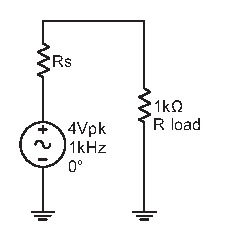
\includegraphics{bjt/unamplified_ac.eps}
\end{center}

\item We've solved the impedance mismatch of the previous part once before, using a op-amp buffer.  Let's see if we can do it with just a transistor!  Connect your signal generator up to the base of the transistor, and connect the load resistor to the emitter.  Sketch the waveform across the load resistor.  Is this a good way to get a 4-volt peak sine wave across the load resistor?
\begin{center}
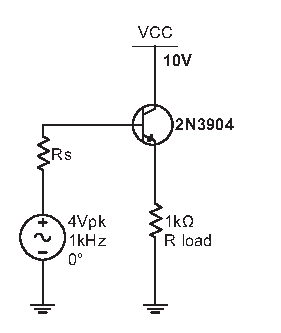
\includegraphics{bjt/ac_with_emit_follower.eps}
\end{center}

\item The circuit above is a lousy amplifier for AC signals, because it cuts off the bottom half of the input signal.  The circuit below shows how to ``bias'' the input signal with a DC voltage so that the base of the transformer is always positive.  What is the voltage at the base of the transistor in the circuit below (AC and DC components)?  Given the values of $R_1$ and $R_2$ shown below, what must be the value of the capacitor for the cutoff frequency $f_C$ to be 100~Hz?  (We're picking $f_C=100$~Hz because we want to be sure that the AC amplitude $V_{OUT}$ is the same as the AC amplitude $V_{IN}$ at 1~kHz.)
\begin{center}
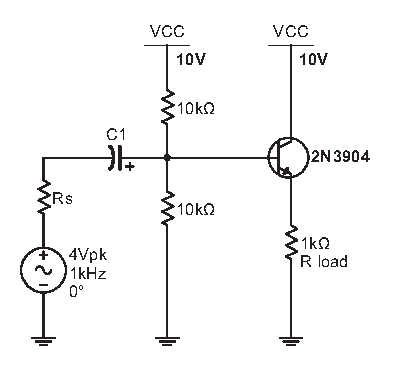
\includegraphics{bjt/emit_follower_biased_input.eps}
\end{center}

\pagebreak[3]
\item Great!  You now have a sinusoidal output that looks like the input.  The only problem is that the output has an additional DC offset you don't especially want.  To eliminate the DC offset from $V_{OUT}$, your first instinct should be to use a high pass filter on the output, as shown below.  Theoretically, what is the cutoff frequency of the output filter shown in the diagram?  Now measure the signal across the load resistor.  Is it consistent with what you expect?  (It might not be....)
\begin{center}
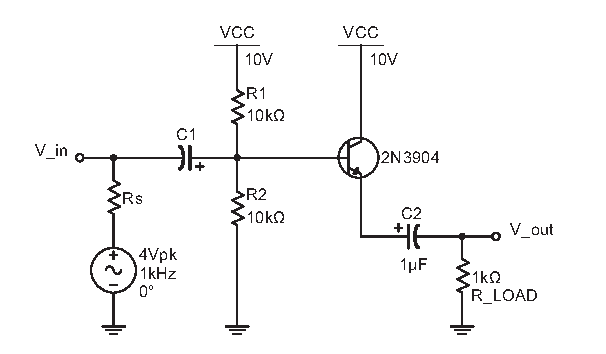
\includegraphics{bjt/biased_output_and_input_incorrect.eps}
\end{center}

\item From the measurements you have just made, you have probably found that the circuit above is totally useless.  It doesn't work, because current can never flow backwards across the transistor; the junction between the base and emitter is a diode, and current only flows across it forwards. Once the capacitor charges up to a maximum voltage, there is no way for it to discharge.  To provide a path for it to discharge, you will need to use a second resistor in parallel with $C_2$ and $R_{LOAD}$, as shown below.  The value of this discharge resistor has to be less than half of the load resistance for this to work properly.  What values of $C_1$ and $C_2$ are required to make this amplifier work well over the entire frequency range of human hearing, from 20~Hz to 20~kHz?  (Be careful, that's a trick question.  Is each of these a high-pass or a low-pass filter?)
\begin{center}
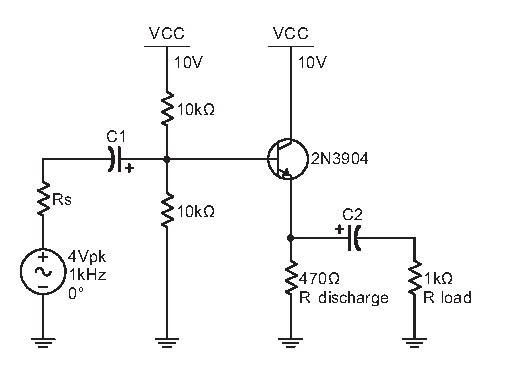
\includegraphics{bjt/biased_output_and_input_correct.eps}
\end{center}

\end{enumerate}

\textbf{Possible Exam Questions:}

\begin{itemize}

\item If you want to use a control voltage to turn the current in another circuit on or off, is it better to use a relay or a bipolar junction transistor?  Discuss the advantages and disadvantages of each.  Topics should include the size of the switching current required (into the transistor base or through the coil of the relay), the size of the load currents that can be controlled, whether you can control both AC and DC load currents, the size of the voltage drop across the relay contacts or between the emitter and collector, switching speed, size, cost, and reliability.  (A bulleted list would be fine.)

\item The circuit you built in the final part of this lab is called an ``emitter-follower amplifier'' or ``common collector amplifier.''  Design an emitter-follower amplifier (from scratch and from memory) with an input impedance of $\ge 10$~k$\Omega$ suitable for $R_{LOAD}=1$~k$\Omega$ and $f=10$~Hz.

\item In the drawing in the final part of this lab, the resistor $R_1$ is changed to 30~k$\Omega$, and the capacitor $C_1$ is 100~nF.  What is the cutoff frequency of this amplifier?

\end{itemize}







